% !TeX spellcheck = en_US
% !TeX root = notes.tex
\subsection{Multimedia}
\subsubsection{Audio}
\begin{itemize}
	\item Analog audio signal sampled at constant rate (telephone: 8000 samples/sec, CD music: 44,100 samples/sec)
	\item quantized, i.e. rounded (8 bits for 256 values)
	\item Example rates (CD: 1.411 Mbps, MP3: 96,128,160 kbps, Internet Telephony: 5.3 kpbs)
\end{itemize}
\subsubsection{Video}
\begin{itemize}
	\item MPEG 1 (CD-ROM) 1.5 Mbps
	\item MPEG 2 (DVD) 3-6 Mbps
	\item MPEG 4 (often used in Internet) <1 Mbps
\end{itemize}
\subsubsection{3 Application Types}
\begin{itemize}
	\item\textbf{Streaming, stored} audio, video
	\begin{description}
		\item[streaming:] can begin playout before downloading entire file
		\item[stored (at server):] can transmit faster than audio/video will be rendered (implies storing/buffering at client)
	\end{description}
	\item\textbf{conversational} voice/video over IP (interactive nature of human-to-human conversation limits delay tolerance
	\item\textbf{streaming live} audio, video
	\item Once playout begins, playback must match original timing (network delays are variable)
	\begin{itemize}
		\item\textbf{Client-side buffer} to match playout requirements
	\end{itemize}
	\item RTP [RFC 2326] multimedia payload types
\end{itemize}

\subsection{Voice-over-IP (VoIP)}
\begin{itemize}
	\item\textbf{VoIP end-end-delay requirement:} needed to maintain ``conversational'' aspect (< 150msec: good, > 400msec bad)
	\item\textbf{session initialization:} how does callee advertise IP address, port number, encoding algorithms?
	\item\textbf{value-added services:} call forwarding, screening, recording
	\item\textbf{emergency services:} 911
	\item\textbf{network loss:} IP datagram lost due to network congestion (router buffer overflow)
	\item\textbf{delay loss:} IP datagram arrives too late for playout at receiver
	\item\textbf{loss tolerance:} depending on voice encoding, loss concealment, packet loss rates between 1\% and 10\% can be tolerated
\end{itemize}
\subsubsection{Adaptive playout delay}
\begin{itemize}
	\item estimate network delay, adjust playout delay at beginning of each talk spurt
	\item silent periods compressed and elongated
\end{itemize}
$$ d_i = (1-\alpha)d_{i-1}+\alpha(r_i-t_i) $$
\begin{description}
	\item[$d_i$:] delay estimate after ith packet
	\item[$\alpha$:] small constant e.g. 0.1
	\item[$r_i$:] time received
	\item[$t_i$:] time sent (timestamp)
\end{description}
\subsubsection{Recovery from packet loss}
\textbf{simple FEC (Forward Error Correction)}
\begin{itemize}
	\item for every group of $n$ chunks, create redundant chunk by exclusive OR-ing $n$ original chunks
	\item send $n+1$ chunks, increasing bandwidth by factor $\frac{1}{n}$
	\item can reconstruct original $n$ chunks if at most one lost chunk from $n+1$ chunks, with playout delay
\end{itemize}
%\subsubsection{Skype}
%\begin{leftbar}
%	Proprietary application-layer protocol (inferred via reverse engineering) $\rightarrow$ encrypted messages
%\end{leftbar}
%\begin{figure}[H]
%	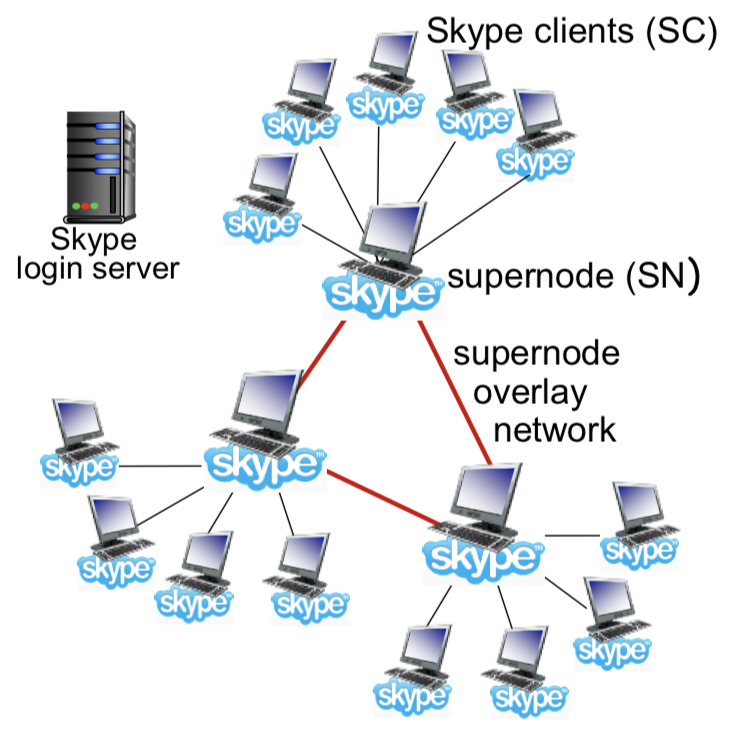
\includegraphics[width=\linewidth]{skype}
%	\centering
%	\caption{Skype Network Layout}
%\end{figure}
%P2P components:
%\begin{description}
%	\item[clients:] Skype peers connect directly to each other for VoIP call
%	\item[super nodes (SN):] Skype peers with special functions
%	\item[overlay network:] among SNs to locate SCs
%	\item[login server]
%\end{description}

\subsection{Real-Time Protocol (RTP)}
\begin{itemize}
	\item RTP specifies packet structure for packets carrying audio, video data
	\item RFC 3550
	\item RTP packet provides
	\begin{itemize}
		\item payload type identification
		\item packet sequence numbering
		\item time stamping
	\end{itemize}
	\item RTP runs in end systems
	\item RTP packets encapsulated in UDP segments
	\item interoperability: if two VoIP applications run RTP, they may be able to work together
\end{itemize}
\subsubsection{RTP runs on top of UDP}
RTP libraries provide transport-layer interface that extends UDP:
\begin{itemize}
	\item port numbers, IP addresses
	\item payload type identification
	\item packey sequence numbering
	\item time-stamping
\end{itemize}
\subsubsection{RTP and QoS}
\begin{itemize}
	\item RTP does \textbf{not} provide any mechanism to ensure timely data delivery or other QoS guarantees
	\item RTP encapsulation only seen at end systems (not by intermediate routers)
	\subitem routers provide best-effort service, making no special effort to ensure that RTP packets arrive at destination in timely matter
\end{itemize}

\subsection{Real-Time Control Protocol (RTCP)}
\begin{itemize}
	\item works in conjuncation with RTP
	\item each participant in RTP session periodically sends RTCP control packets to all other participants
	\item each RTCP packet contains sender and/or receiver reports
	\subitem report statistics useful to application: \# packets sent, \# packets lost, interarrival jitter
	\item feedback used to control performance
	\subitem sender may modify its transmissions based on feedback
\end{itemize}
\subsubsection{RTCP: packet types}
\begin{description}
	\item[receiver report packets:] fraction of packets lost, last sequence number, average interarrival jitter
	\item[sender report packets:] SSRC of RTP stream, current time, number of packets sent, number of bytes sent
	\item[source description packets:] email address of sender, sender's name, SSRC of associated RTP stream. Provide mapping between the SSRC and the user/host name
\end{description}

\subsection{SIP: Session Initiation Protocol}
\textbf{long-term vision:}
\begin{itemize}
	\item all telephone calls, video conference calls take place over Internet
	\item people identified by names or e-mail addresses, rather than by phone numbers
	\item can reach callee (if callee so desires), no matter where callee roams, no matter what IP device callee is currently using
\end{itemize}
\subsubsection{SIP services}
\begin{itemize}
	\item SIP provides mechanisms for call setup:
	\begin{itemize}
		\item for caller to let callee know she wants to establish a call
		\item so caller, callee can agree on media type, encoding
		\item to end call
	\end{itemize}
	\item determine current IP address of callee: maps mnemonic identifier to current IP address
	\item call management:
	\begin{itemize}
		\item add new media streams during call
		\item change encoding during call
		\item invite others
		\item transfer, hold calls
	\end{itemize}
\end{itemize}
\textit{SIP default port 506}\\
\textbf{SIP registrar}\\
Function of SIP server (registrar). When Bob starts SIP client, client sends SIP REGISTER message to Bob's registrar server\\
\textbf{SIP proxy}\\
Function of SIP server (proxy). Alice sends invite message to her proxy, proxy responsible for routing SIP messages to callee possibly through multiple proxies. Bob sends response back through same set of SIP proxies, proxy returns Bob's SIP response message to Alice. SIP proxy analogous to local DNS server plus TCP setup

\begin{note}{Comparison with H.323}
	\begin{itemize}
		\item Another signaling protocol for real-time, interactive multimedia
		\item Complete, vertically integrated suite of protocols for multimedia conferencing; signaling, registration, admission control, transport, codecs
		\item SIP is a single component. Works with RTP, but does not mandate it. Can be combined with other protocols, services
		\item SIP uses KISS principle
	\end{itemize}
\end{note}